\section{Aufteilung}
\subsection{Geplante Aufteilung}
Im Folgenden ist eine Grafik zu sehen, die einen Überblick über die Implementierung des MatFlow Systems gibt. 
Eine detailliertere Ansicht über die Aufgabenteile findet man im \nameref{Anhang}.
\vspace{0.3in}
\begin{figure}[H]
    \centerline{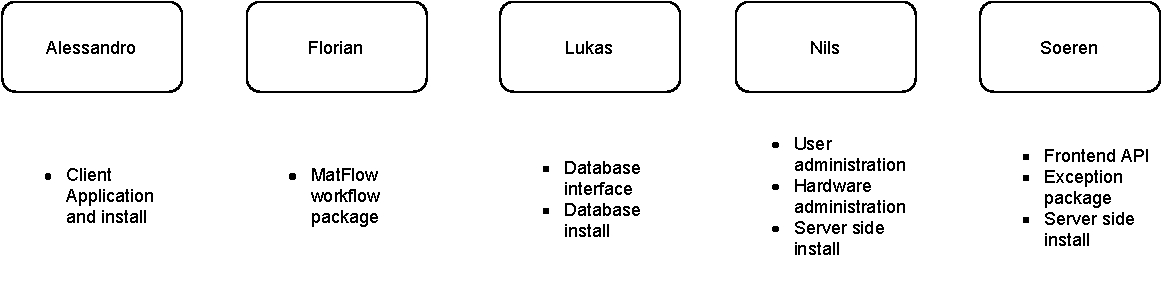
\includegraphics[scale=0.8]{res/aufteilung.pdf}}
    \caption{Aufteilung}
    \end{figure}

\subsection{Endgültiger Stand nach Implementierung}
Frontend
\begin{itemize}
    \item \textbf{Jede} der anzuwählenden Seiten ist implementiert
    \item Alle benötigten Datenklassen sind voll funktionsfähig implementiert
\end{itemize}
Frotend API
\begin{itemize}
    \item \textbf{Jede} der zur Verfügung stehenden Methoden ist bis auf die \nameref{Cookie} voll funktionsfähig implementiert
    \item Alle Unit Tests sind geschrieben
\end{itemize}
User Administration
\begin{itemize}
    \item \textbf{Jede} der zur Verfügung stehenden Methoden ist voll funktionsfähig implementiert
    \item Alle Unit Tests sind geschrieben
\end{itemize}
Hardware Administration
\begin{itemize}
    \item \textbf{Vile} der zur Verfügung stehenden Methoden ist voll funktionsfähig implementiert
\end{itemize}
Workflow Package
\begin{itemize}
    \item \textbf{Jede} der zur Verfügung stehenden Methoden ist voll funktionsfähig implementiert
    \item Alle Unit Tests sind geschrieben
\end{itemize}
Exception package
\begin{itemize}
    \item \textbf{Jede} der zur Verfügung stehenden Methoden ist voll funktionsfähig implementiert
    \item Alle unittests sind geschrieben.
\end{itemize}
Database package
\begin{itemize}
    \item Der Großteil der zur Verfügung stehenden Methoden ist voll funktionsfähig implementiert
\end{itemize}
Zu implementieren bleibt noch
\begin{itemize}
    \item Die request Klasse BackendCommunicator und Unit Tests im Frontend
    \item Die WorkflowData Schnittstelle im Database package
    \item Der alternierende Operator für airflow
    \item Die containerweise Ausführung der Serverapplikation im Backend (Nomad Job File)
\end{itemize}